\section{Evaluation}
\label{sec:semnotesevaluation}

We conducted a task-based summative user evaluation, comparing SemNotes to the popular note-taking application Evernote\footnote{\url{http://evernote.com/}}. The goal of the experiment was to determine whether the effort required for the creation of links between notes and resources is repaid by easier search. Towards this goal, we measured the effort needed to execute the same set of tasks with both tools, and compared the results. We used time spent, number of mouse clicks and number of key presses, as measures for effort. After the experiment, we asked the participants about their experience in a questionnaire.

The two applications compared have the same main functionality, note-taking. We chose Evernote as baseline, as it is a very popular note-taking tool that is freely available. Its set of functionalities are richer than those of SemNotes, but the basic features are present and similar in both applications. The feature that distinguishes SemNotes is the same that we want to measure---the creation of links between the notes and desktop resources, based on suggestions given by the application. SemNotes runs on KDE on Linux, and uses the framework provided by Nepomuk-KDE Semantic Desktop. Evernote runs on several operating systems for desktop and mobiles, but Linux is not one of them, therefore we used its Windows version. 

Evaluation is one of the challenges for application design on the Semantic Desktop. Adding to the challenges of evaluating PIM applications with regards to finding appropriate data and tasks for significant measurements, discussed in \cite{Kelly2006}, semantic PIM applications have the difficulty of lacking equivalent semantic tools for a one-on-one comparison. That is why for this evaluation, we followed a methodology similar to the ones described in \cite{Elsweiler2007} and \cite{Franz2009}, of comparing our semantically enabled SemNotes, to a conventional application.

One aspect that we did not evaluate as part of this study is the effect of having the notes connected to the relevant desktop resources from the other applications using the respective resources --- for example, would the extra information from the notes provide an advantage when using a task manager application, and seeing all the linked notes when looking at a task. Such a study would require a longer duration, and also a richer ecosystem of semantic applications, which make use each other's data.

\subsection{Participants} 

Twenty participants took part in the evaluation, all members of our research institute. They are researchers in the field of Semantic Web, thus possibly favouring the semantic application. This bias (if it exists) would however influence only their responses in the questionnaire and not the measured values. Fourteen participants regularly use note-taking and five of them use Evernote as their preferred note-taking tool. None of the participants used Linux as their operating system. Their familiarity with one environment and one application could have influenced the measured results, in favour of Evernote.

\begin{figure}[htb]
 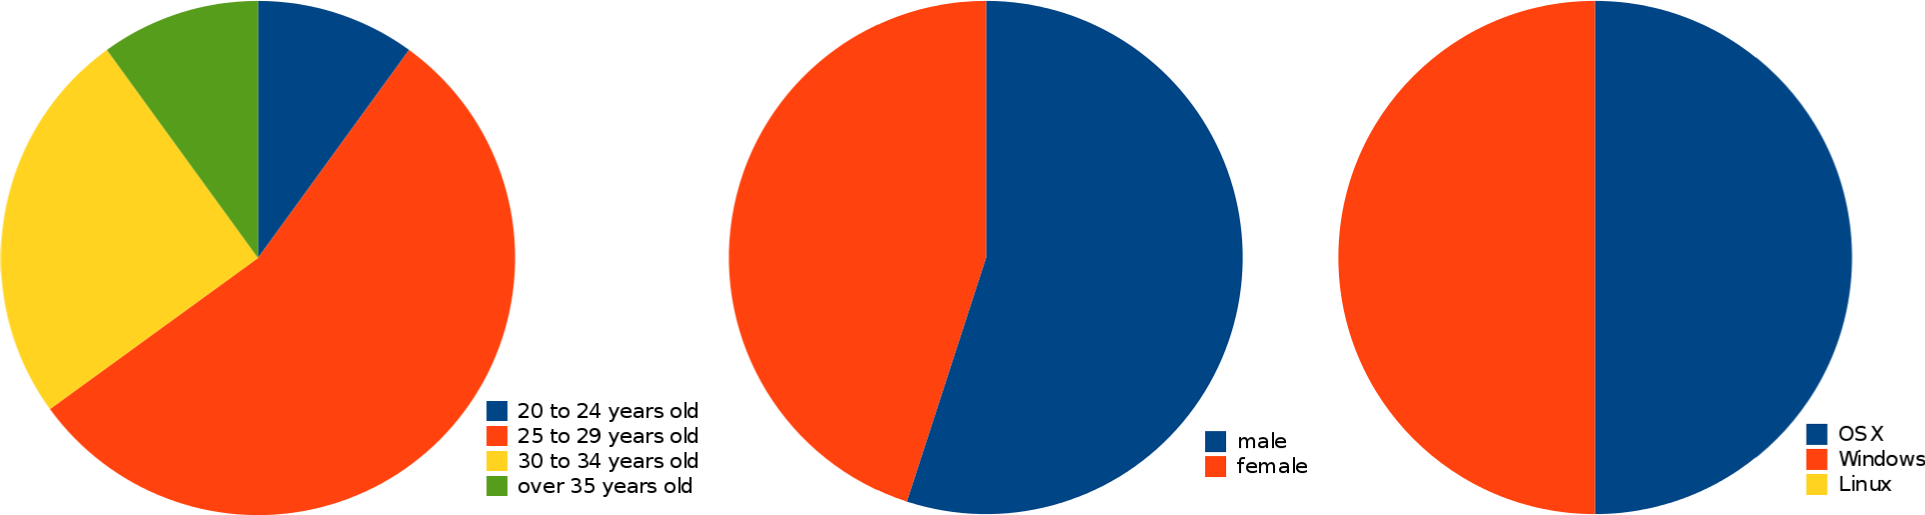
\includegraphics[width=0.95\linewidth]{chapters/core/img/distribs}
\caption{Age, gender and OS distributions of participants.}
\label{fig:distribs}
\end{figure}

Some additional demographic details of the participants: gender distribution was close to even (eleven men and nine women); most of them were in the age groups between 25 and 29 (eleven, equivalent to 55\%), and between 30 and 34 (five, or 25\%). There were seven Master's students, seven Ph.D. students, five senior researchers and one intern. For demographic distributions see Figure \ref{fig:distribs} and Figure \ref{fig:genderdistribs}.

\begin{figure}[htb]
 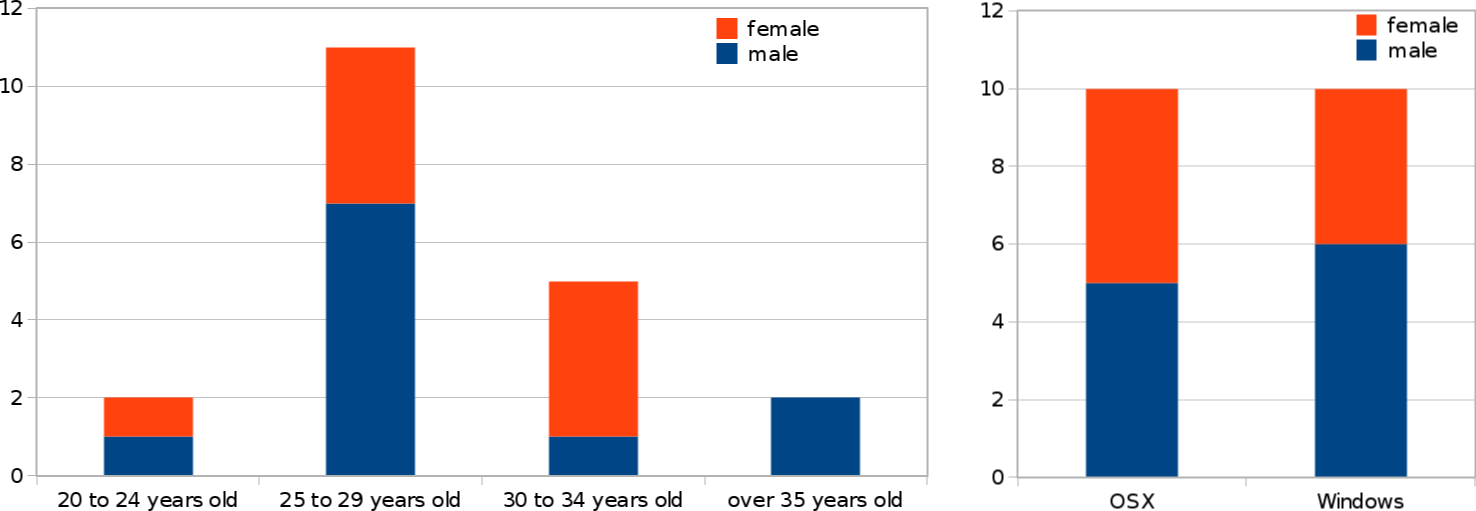
\includegraphics[width=0.9\linewidth]{chapters/core/img/genderdistribs}
\caption{Age and OS distributions of participants per gender.}
\label{fig:genderdistribs}
\end{figure}

\subsection{Data} 

We used two virtual machines for the experiment, preloaded with identical data. To reduce the artificialness of the study, we chose general data familiar to the participants, to which they have access in their everyday work. The dataset contained contact information for 130 members of our institute; 655 recent emails from our mailing lists; 20 scientific papers authored by our colleagues; and photographs from institute events. The note data was also identical: 50 notes on a variety of topics, personal or work-related, tagged with 23 tags. In SemNotes, we also provided links between the notes and the resources mentioned in them: people, projects, events or other notes, within reasonable limits we expect users to interlink their notes (i.e. minimum 0 links, maximum 10 links, average 1.8, median 1). The majority of connections were made to people mentioned in the notes.

\subsection{Tasks} 

We prepared a set of eight tasks. Each participant was requested to run all the tasks in each of the two environments. To prevent order effects from influencing the results, half of the participants started with SemNotes and the other half with Evernote.

\begin{description}
 \item[T1.] Find what information is available about yourself (contact information, documents, emails, photographs)
 \item[T2.] Find the paper titled ``Bridging the Gap between Linked Data and the Semantic Web''. Who are the authors?
 \item[T3.] Find notes tagged with ``todo''.
 \item[T4.] Find to-dos that are related to our institute.
 \item[T5.] Find a to-do related to a presentation by a colleague John.
 \item[T6.] Take a note about planning a social event for your research group. Write the names of two people that have already confirmed. Annotate the note as you see fit.
 \item[T7.] Find a note containing the minutes from the last meeting about a given project. Change the date of the next meeting planned.
 \item[T8.] Take a new note for the action item assigned to you at the last meeting of the project. The action item is in the meeting minutes previously edited, and it requires drafting a document using a paper authored by a colleague. Annotate the note.
\end{description}

The first two tasks were intended to help the participants get accustomed with the data available and the environment; we did not include the time spent on these tasks in the results. 

The last six tasks were focused on note-taking, and their complexity increased gradually. T3, T4, and T5 are search and filter tasks (S), from the very simple to the complex. T6 and T8 are editing tasks (E), including any annotations that the participants made on the notes. T7 is both a search and edit task (SE). It prepares the participants for the most complex search and edit task, T8, which required interaction with the rest of the system (i.e. finding the required paper).

\subsection{Measurements} 

The participants were recorded while doing the tasks of the experiment, and the videos were used to extract the measurements used in the analysis. 
For each task we measured the effort in seconds spent, and number of mouse clicks. 
We also counted the number of key strokes for the tasks involving creation of notes, and we used this measure to normalise the values for time. 
Although we had two separate measures for each task, we were interested in the difference between these values, computed according to:
$$
value_{difference} = value_{SemNotes} - value_{Evernote}
$$
Thus, a positive value means that the value recorded for SemNotes is bigger than the corresponding value for Evernote, and a negative value means that the value for SemNotes is smaller. 

For the time measurements, the time difference represents the extra \emph{effort} required for annotating the notes with links in the editing tasks. For the search tasks the difference shows which of the applications enables the users to find the notes easier, thus the \emph{benefit}. We must specify here that actual searches done by the software were considered instantaneous, as the datasets are small and we did not intend to measure the performance of the search algorithms used.

For the number of mouse clicks, the difference represents the extra \emph{effort} required, for both types of tasks.

\begin{figure}[tb]
\begin{center}$
 \begin{array}{ccc}
  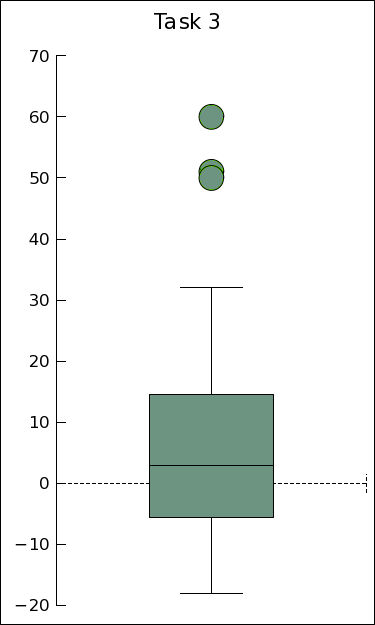
\includegraphics[width=0.29\linewidth]{chapters/core/img/task3difboxplot} &
  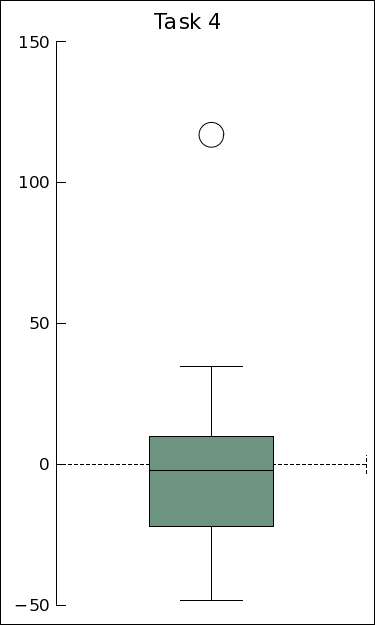
\includegraphics[width=0.29\linewidth]{chapters/core/img/task4difboxplot} &
  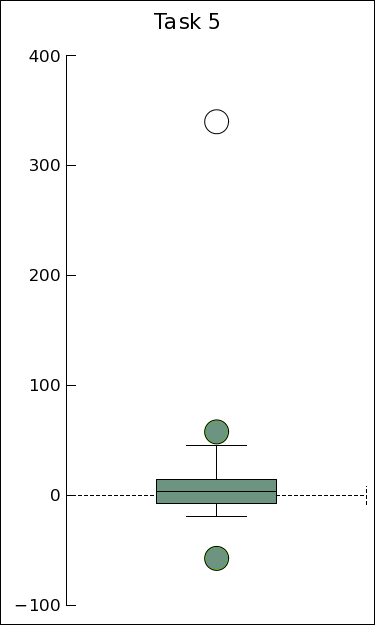
\includegraphics[width=0.29\linewidth]{chapters/core/img/task5difboxplot} \\ 
  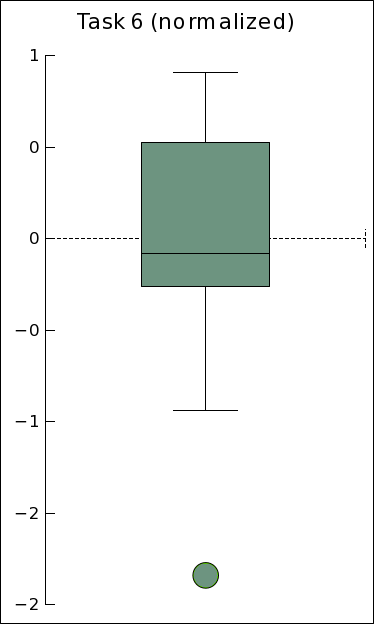
\includegraphics[width=0.29\linewidth]{chapters/core/img/task6difboxplot} &
  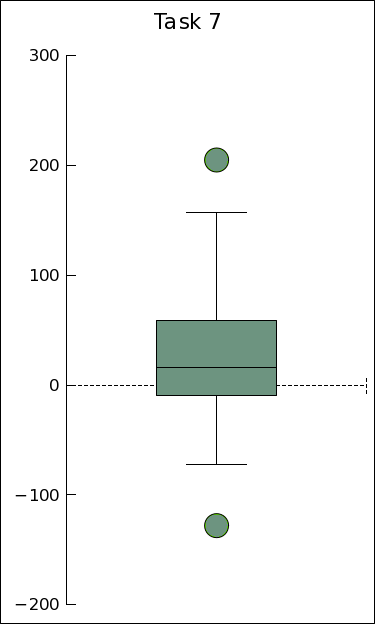
\includegraphics[width=0.29\linewidth]{chapters/core/img/task7difboxplot} &
  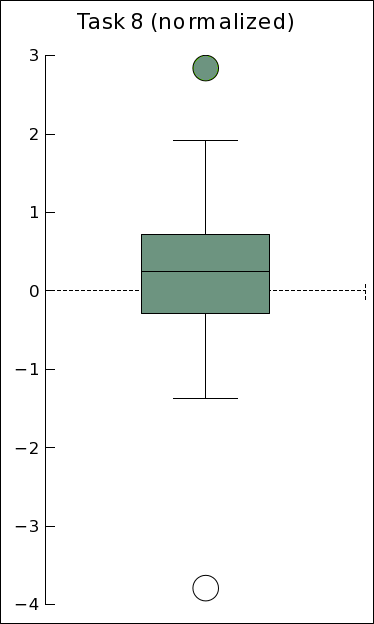
\includegraphics[width=0.29\linewidth]{chapters/core/img/task8difboxplot} 
 \end{array}$
\end{center}
\caption{Inter-quartile ranges for the time difference.}
\label{fig:boxplots}
\end{figure}

After a first analysis of the results, we noticed that some values for time were unrealistically high or low. They coincided with the measurements when the participants stopped to ask a question or comment on a feature. We decided to eliminate these outlier values by using only the measurements that fall in the inter-quartile range, for all tasks --- see Figure \ref{fig:boxplots}.

\subsection{Quantitative Results}

We tested if the effort measured in time and mouse clicks was different when using SemNotes than when using Evernote. Table \ref{tab:semnotesresults} shows the results, with the statistically significant values in bold (\begin{math}p < 0.05 \end{math}).

\begin{table}[htp]
\centering
\ra{1.3}
\begin{tabular}{@{}clcr@{.}lr@{.}lr@{.}lcr@{.}lr@{.}lr@{.}l}
\toprule
\multirow{2}{*}{\textbf{T}} &&& \multicolumn{6}{c}{\textbf{Time (s)}} && \multicolumn{6}{c}{\textbf{Clicks}} \\

&&& \multicolumn{2}{c}{\textbf{Avg}} & \multicolumn{2}{c}{\textbf{Med}} & \multicolumn{2}{c}{\textbf{\textit{t}}} && \multicolumn{2}{c}{\textbf{Avg}} & \multicolumn{2}{c}{\textbf{Med}} & \multicolumn{2}{c}{\textbf{\textit{t}}} \\
\midrule
\textbf{T3} & (S) && 0 & 5 & 0 & 0 & 0 & 152 && 0 & 167 & 0 & 0 & 0 & 692 \\

\textbf{T4} & (S) && -8 & 0 & -8 & 0 & \textbf{-2} & \textbf{94} && -0 & 333 & -1 & 0 & -0 & 48 \\

\textbf{T5} & (S) && -0 & 125 & 1 & 0 & -0 & 046 && 0 & 857 & 1 & 0 & 1 & 426 \\

\textbf{T6} & (E) && 0 & 063 & 0 & 016 & 0 & 486 && 6 & 067 & 8 & 0 & 2 & 026 \\

\textbf{T7} & (SE) && 14 & 357 & 13 & 0 & 1 & 713 && 4 & 812 & 2 & 0 & 1 & 527 \\

\textbf{T8} & (SE) && 0 & 249 & 0 & 243 & 1 & 004 && 20 & 8 & 12 & 0 & \textbf{3} & \textbf{08} \\

\bottomrule
\end{tabular} 
\caption{Statistics for time and click differences.}
\label{tab:semnotesresults}
\end{table}

Results show that for the simple search task T3 the difference is positive, which suggests that it takes longer to finish the task with SemNotes. However, the difference is not significant. For the complex search tasks that follow, T4 and T5 the difference has negative values, showing that the users spent less time on complex searches when using SemNotes, thus supporting the claim that the use of interlinked data makes notes easier to find. Only the results for T4 are statistically significant. None of the measures of number of mouse clicks for the search tasks are statistically significant, the differences being in average less than 1 click, with a median value of 0, -1 and +1 respectively for the tasks T3, T4 and T5.

For the editing task T6, the values are positive, thus it took longer to finish it with SemNotes. This was expected, as in SemNotes there is the additional step of annotating the notes with links to desktop resources. However, the differences are very close to 0 (0.063s average and 0.016s median) and not statistically significant. This editing task did require in average 6 more mouse clicks in SemNotes, with a median value of 8, but the difference is also not statistically significant.

For the more complex search and edit tasks T7 and T8, the time differences, while positive, thus in favour of Evernote, are not significant. For both tasks the values were positive, which mean more clicks when using SemNotes. However, task T8, that required creating and annotating a complex note based on information from other sources, had statistical significant difference in number of clicks, in favour of Evernote (more clicks needed in SemNotes). 

The positive difference in the number of clicks required for all editing tasks (T6, T7 and T8) is not surprising, as the participants recognised the value of creating links and proceeded to link the new note to the relevant resources. This was however a motivation for providing better keyboard support for the annotation of notes in the future version of the tool.

In summary, the results show that there are significant improvements (for one of two tasks) in the time spent on complex searches, when the data is interlinked, at no significant extra cost for the creation of the links. Linking does however significantly increase the effort measured by number of mouse clicks (for one of two tasks).

\subsection{Questionnaire}

We asked the participants to fill in an anonymous questionnaire related to the experiment. The questionnaire is listed in Appendix~\ref{ap:questionnaire}. According to the answers, on a scale from 1 to 5, the tasks were simple (mean 2.25) and similar to the ones in their daily work (mean 3.4), and the data provided was familiar (mean 3.2). 

The answers also show that 60\% of the participants (12) felt that SemNotes helped them finish the tasks \emph{faster}, while only 20\% (4) said Evernote, and 20\% did not feel any difference between the tools. When asked which of the two applications helped them perform the tasks \emph{better}, 80\% of the participants chose SemNotes, while the remaining 20\% did not feel that there was any difference (see Figure \ref{fig:betterfaster} for a graphical representation).

\begin{figure}[htb]
 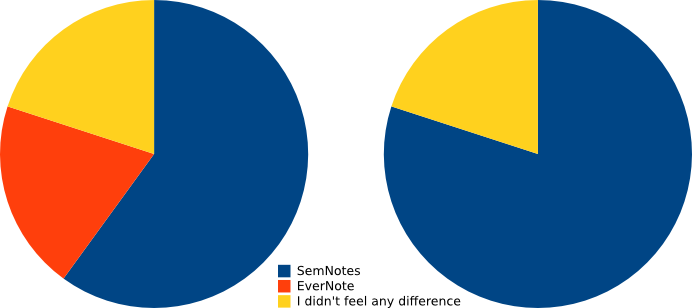
\includegraphics[width=0.7\linewidth]{chapters/core/img/fasterbetter}
\caption{Which tool helped perform the tasks faster (left) and better (right).}
\label{fig:betterfaster}
\end{figure}

The participants had a good overall impression of SemNotes (with a mean of 4.15 on a scale from 1 to 5). This rating was supported by comments like ``\emph{That was cool.}'', and requests for SemNotes for other operating systems: ``\emph{Maybe you could make an OS X version?}'' and ``\emph{When is a port for Windows 7 coming?}''.

The semantic annotation was one of the most liked features of SemNotes, and one of the features most missed in Evernote, according to the questionnaire. Another advantage of SemNotes was considered the multiple filtering by mixed criteria, with several participants considering it the best feature. The rating of notes was listed as the least liked feature of SemNotes by three participants. The tag cloud was the most controversial feature, as many participants liked it and found it very useful, while others would have preferred a simple list of tags: ``\emph{Usually I don't like tag clouds, but the one in SemNotes was really useful.}'' and ``\emph{While the tag cloud helps in determining the most used tag, a simple list with the tags seems to be easier to search.}'' 
